% little trick to replace lib.tex by this
\renewcommand{\doctitle}[1]{
	\chapter{#1}
}
\renewcommand{\biblio}[1]{}
\doctitle{Conception du Voltage-Controlled-Oscillator (VCO)}

\section{Blocs fonctionnels}
Pour réaliser le VCO, nous avons décidé d'utiliser 3 blocs
fonctionnels : un intégrateur, un soustracteur et un
comparateur à hystérésis (ou trigger de Schmitt). Ces blocs
fonctionnels sont agencés comme sur la figure \ref{fig:blocs}.

\begin{figure}[ht]
	\centering
	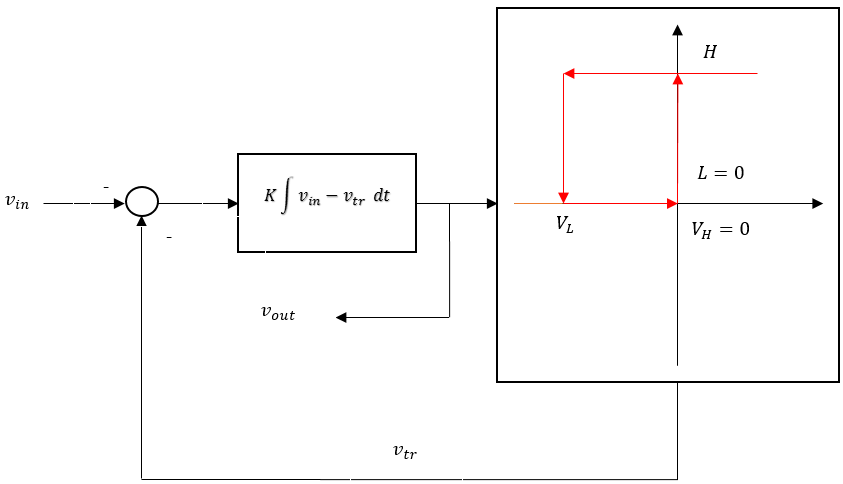
\includegraphics[scale=0.85]{img/blocs-fonctionnels.png}
	\caption{Schéma en blocs fonctionnels de notre VCO.}
	\label{fig:blocs}
\end{figure}

Sur cette figure, $V_L$ et $V_H$ désignent les tensions de
basculement du trigger tandis que $H$ et $L$ désignent
les valeurs possibles pour $v_{\text{tr}}$, la tension de sortie
du trigger. On peut se convaincre que cet agencement de blocs
fonctionnels remplit bien la fonction d'oscillateur contrôlé en tension. 

Pour cela, considérons $v_{\text{tr}}$ initialement à \unit{0}{\volt}
et $v_{\text{in}} = x$ avec $x > 0$. On a alors dans un premier temps
\begin{equation}
	v_{\text{out}} = K\int x - 0 \dif t = Kxt.
	\label{eq:croiss}
\end{equation}
Cette droite de pente positive est directement plus grande que $V_H = 0$
et on a donc directement $v_{\text{tr}} = H$. La tension de sortie
devient alors
\begin{equation}
	v_{\text{out}} = K\int x - H \dif t = K(x-H)t.
	\label{eq:decroiss}
\end{equation}
En supposant que $H$, la tension de saturation du trigger, est largement
plus grande que $x$, on a maintenant une droite avec une pente
très négative qui va atteindre $V_L$ en un temps $t_f$ négligeable.
Une fois ce temps très court passé, et donc $V_L$ atteint, on aura
à nouveau $v_{\text{tr}} = 0$ et donc à nouveau la droite de
l'équation \ref{eq:croiss}. La signal $v_{\text{out}}$ de sortie
est un signal \textbf{en dent de scie} dont la période est
égale au temps $t_r$ mis par la droite de l'équation \ref{eq:croiss}
pour passer de $V_L$ à $V_H = 0$ 
\[ T = \frac{V_L}{Kv_\text{in}}. \]
On a donc une fréquence directement proportionnelle $v_\text{in}$ à
selon
\[ f = \frac{K}{V_L}v_\text{in}. \]

\section{Circuit et simulations}
Pour implémenter le circuit équivalent à ces blocs fonctionnels,
on peut combiner le soustracteur et l'intégrateur afin
de réduire à deux le nombre de blocs nécessaire. Une façon
d'implémenter ce circuit est représentée à la figure
\ref{fig:circuit}.

En pratique, un problème apparait lorsqu'on
simule ce circuit. Pour une raison inconnue,
la tension ``basse'' du trigger ($L$ sur le schéma
en blocs fonctionnels) est de l'ordre de 
\unit{150-300}{\milli\volt}\footnote{Et ce même
lorsque le trigger est déconnecté du reste du circuit.}.
On peut observer cet effet sur la figure \ref{fig:simulation},
qui présente les résultats de simulation.
On verra par la suite que cela entraîne quelques
difficultés.

On peut maintenant exprimer $v_{\text{out}}$ en terme
des composants du circuits. A la sortie de l'intégrateur/soustracteur,
on a
\begin{equation}
	v_{\text{out}} = \frac{1}{RC} \int -v_{\text{in}} - v_{\text{tr}} \dif t 
	\label{eq:eq-circ}
\end{equation}
où $v_{\text{tr}}$ vaut $L$ ou $H$ et avec $v_{\text{in}} < 0$.
% TODO
%Vérifions que ce circuit
%remplit également le rôle de VCO. On démarre avec $v_{\text{tr}} = L$
%et $v_{\text{in}} = x < 0$. L'équation \ref{eq:eq-circ} devient
%donc dans un premier temps
%\begin{equation}
	%v_{\text{out}} = \frac{1}{RC} \int -x-L \dif t. 
%\end{equation}

On trouve un temps de montée $t_r = \frac{V_LRC}{v_{\text{in}} + L}$
et un temps de descente $t_f = \frac{-V_LRC}{v_{\text{in}} + H}$.
Si l'entrée est suffisamment faible par rapport à $H$, on
peut négliger $t_f$ et on obtient alors
\[ T = \frac{V_LRC}{v_{\text{in}} + L} \]
ou encore
\[ f = \frac{v_{\text{in}} + L}{V_LRC} \]
où $V_L = -\frac{R_1}{R_2}V_{CC}$.

On peut vérifier que la simulation et le calcul fournissent
bien le même résultat pour le circuit donné à la figure \ref{fig:circuit}
et les résultats de simulation donnés à la figure \ref{fig:circuit}.
Par calcul, on obtient une période de \unit{0.306}{\milli\second}
tandis que les mesures sur les graphes de simulation indiquent
une période de \unit{0.30}{\milli\second}\footnote{On a donc une
erreur relative de l'ordre de 2\%, sans doute dû aux imprécisions
de mesures.}.

La fréquence en fonction de $v_{in}$ est représentée à la figure
\ref{fig:f-vs-vin}. Afin de garder une tension de sortie
en dents de scie, on ne peut pas trop augmenter $v_{in}$ (car
on finirait par obtenir un triangle). On ne peut pas non
plus prendre une valeur trop petite pour $v_{in}$ car notre
VCO ne fonctionne plus si $-v_{in} < L$. En fixant
la valeur minimale de la tension d'entrée à \unit{-300}{\milli\volt} et la valeur
maximale à \unit{-1.6}{\volt} (de manière arbitraire, mais
de façon à garder un signal en dents de scie), on devrait
\textbf{théoriquement} (insistons sur ce mot) pouvoir générer 
des fréquences allant de \unit{100}{\hertz} à \unit{2}{\kilo\hertz}.

\begin{figure}[ht]
	\centering
	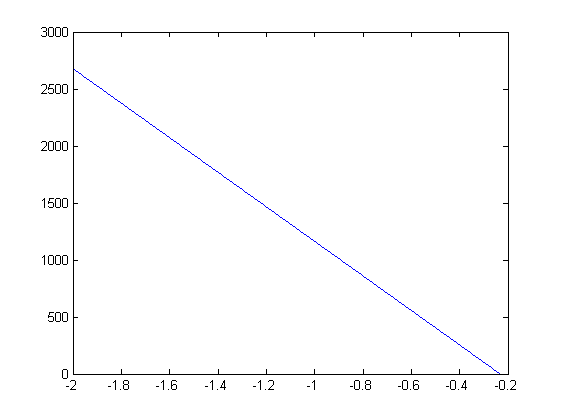
\includegraphics[scale=0.65]{img/freq-vs-vin.png}
	\caption{Graphe de la fréquence en fonction de la tension d'entrée.}
	\label{fig:f-vs-vin}
\end{figure}

\begin{figure}[ht]
	\centering
	\rotatebox{90}{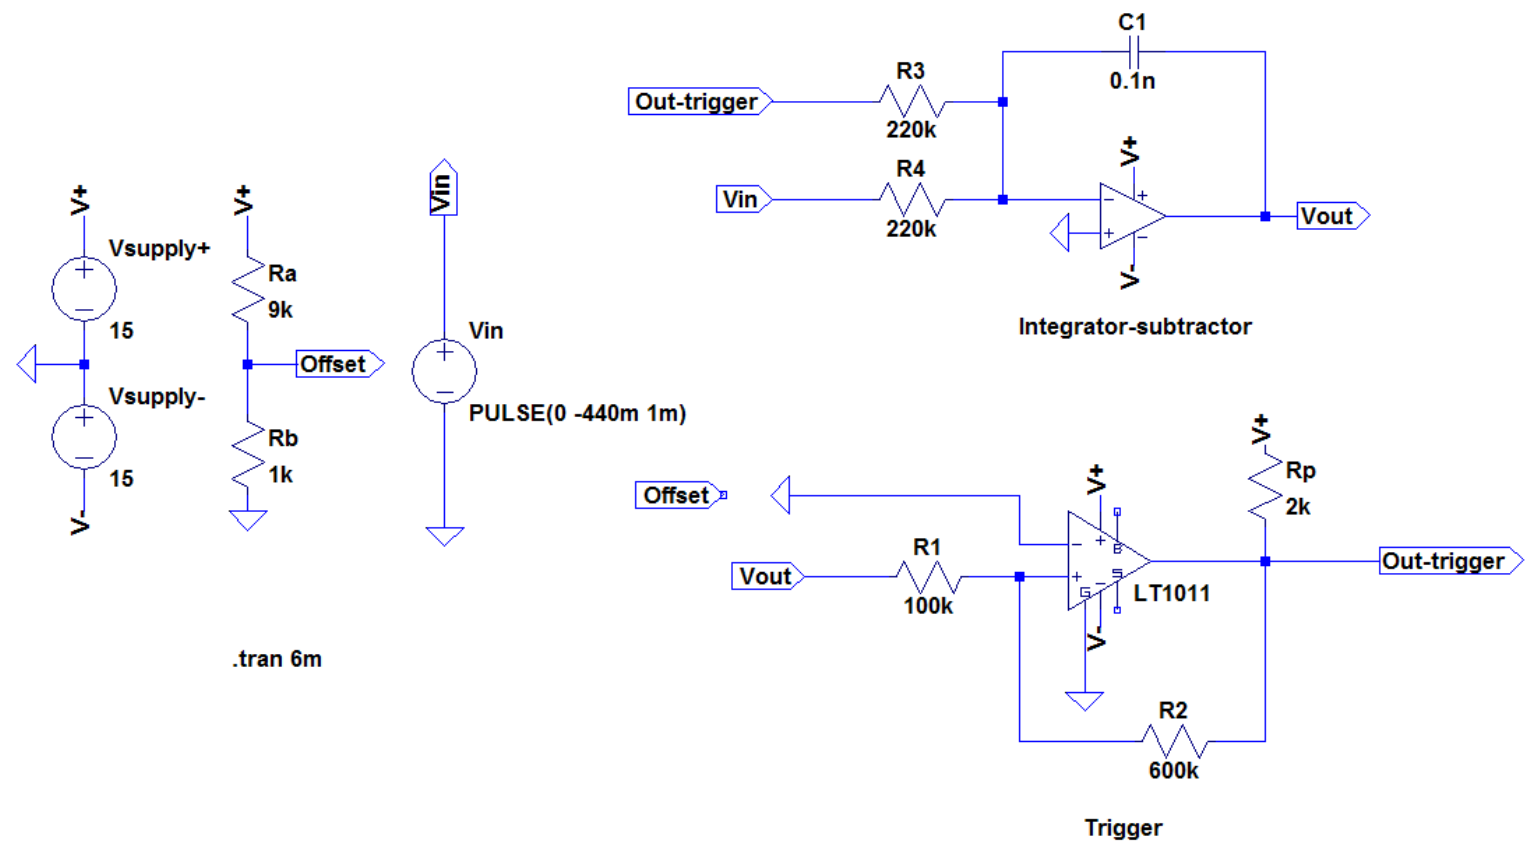
\includegraphics[scale=0.7]{img/circuit.png}}
	\caption{Circuit de notre VCO.}
	\label{fig:circuit}
\end{figure}

\begin{figure}[ht]
	\centering
	\rotatebox{90}{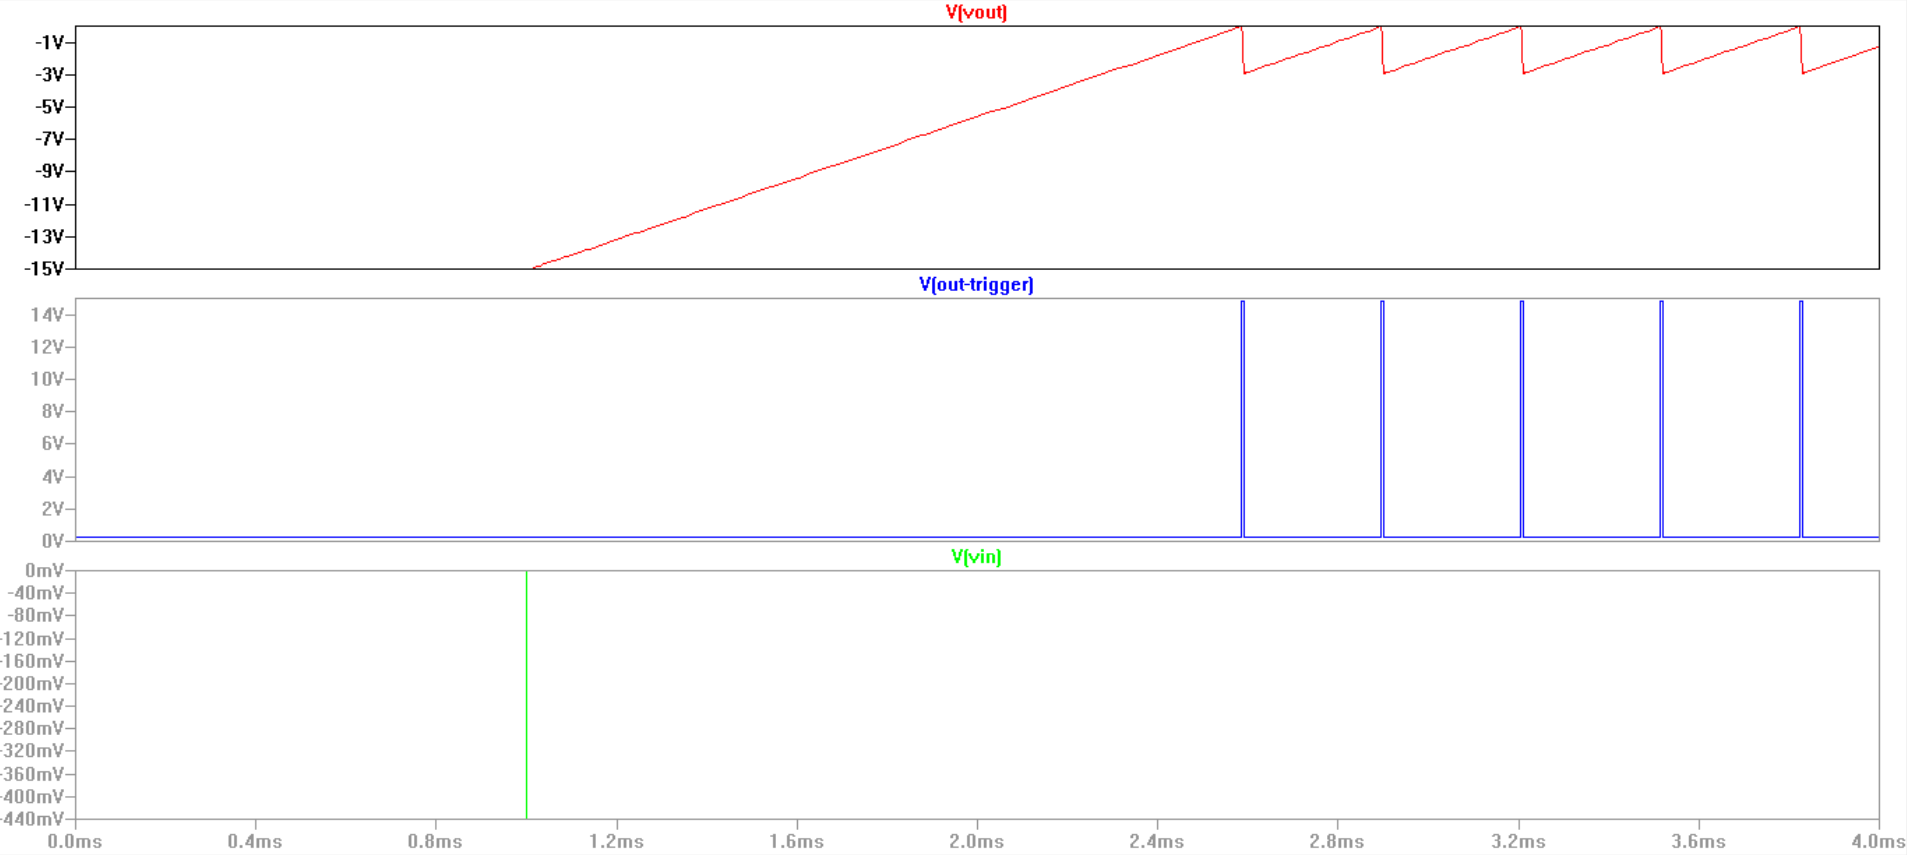
\includegraphics[scale=0.55]{img/simulation.png}}
	\caption{Simulation du circuit de notre VCO. L'entrée est un échelon
	passant de \unit{0}{\volt} à \unit{-440}{\milli\volt}, la sortie
	est un signal en dent de scie, et la sortie du trigger est un train
	d'impulsions.}
	\label{fig:simulation}
\end{figure}

\newpage

\section{Circuit et mesures}
En montant le circuit proposé dans la section précédente, on
constate que $L$ une valeur qui passe de \unit{100}{\milli\volt} à \unit{220}{\milli\volt} (voir figure \ref{fig:trigger-L}).

\begin{figure}[ht]
	\centering
	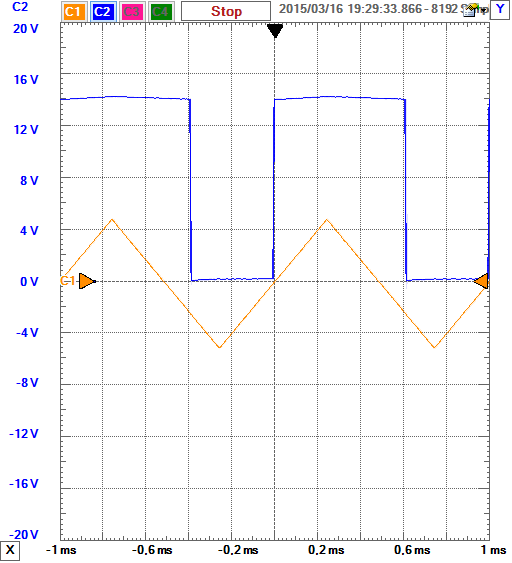
\includegraphics[scale=0.7]{img/trigger-L.png}
	\caption{Test du trigger séparé du reste du circuit.}
	\label{fig:trigger-L}
\end{figure}

La figure \ref{fig:test-440} présente le résultat des mesures sur le circuit 
réel de notre VCO pour une entrée de \unit{-440}{\milli\volt}. Notons 
que les valeurs des résistances ne sont pas les mêmes que celle
utilisée lors de la simulation pour des raisons pratiques (le
schéma du circuit tel que construit est repris sur la
figure \ref{fig:circuit-reel}.

\begin{figure}[ht]
	\centering
	\rotatebox{90}{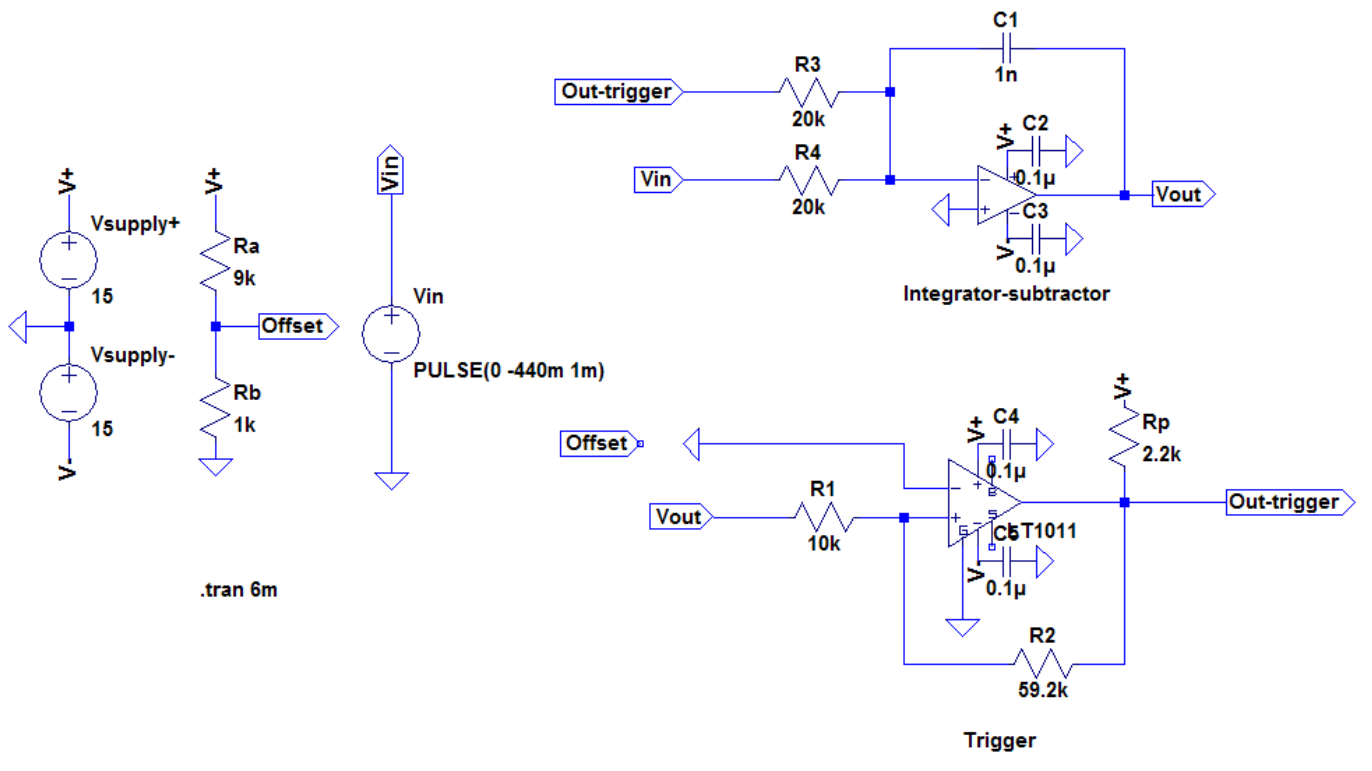
\includegraphics[scale=0.7]{img/circuit-reel.png}}
	\caption{Schéma du circuit tel que construit.}
	\label{fig:circuit-reel}
\end{figure}

\begin{figure}[ht]
	\centering
	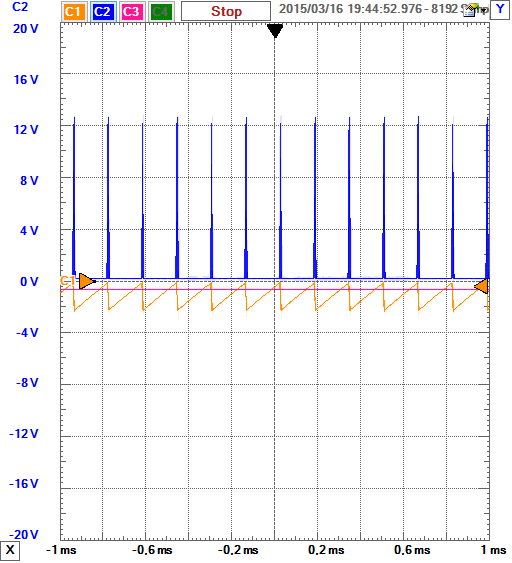
\includegraphics[scale=0.7]{img/circuit-test-440mv.png}
	\caption{Test du circuit.}
	\label{fig:test-440}
\end{figure}

Les figure suivantes montrent les résultats pour
différentes valeurs d'entrées.

\begin{figure}[ht]
	\centering
	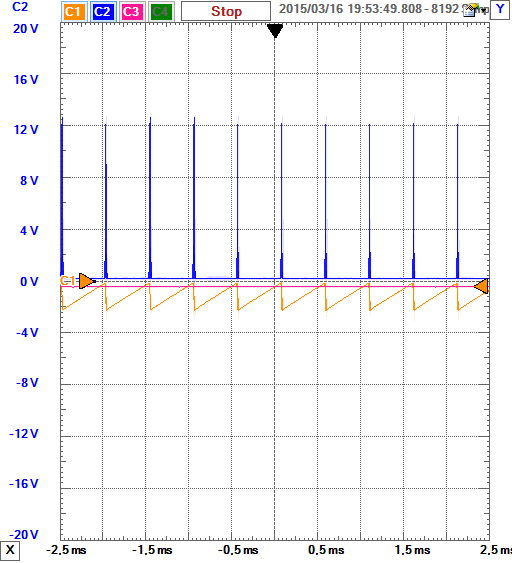
\includegraphics[scale=0.7]{img/circuit-test-260mv.png}
	\caption{Test du circuit pour \unit{-260}{\milli\volt}.}
	\label{fig:test-260}
\end{figure}

\begin{figure}[ht]
	\centering
	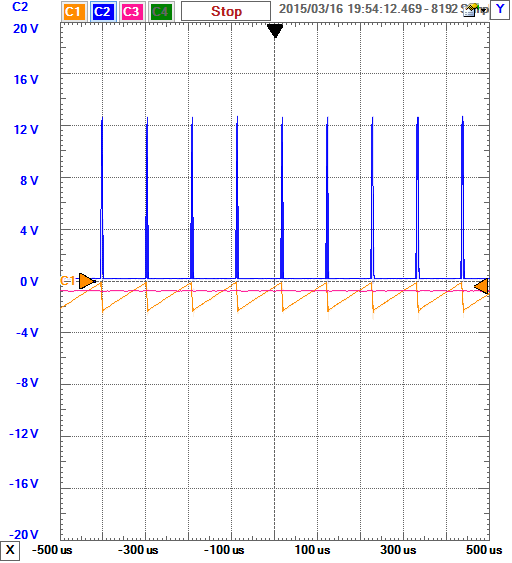
\includegraphics[scale=0.7]{img/circuit-test-580mv.png}
	\caption{Test du circuit \unit{-580}{\milli\volt}.}
	\label{fig:test-580}
\end{figure}

\begin{figure}[ht]
	\centering
	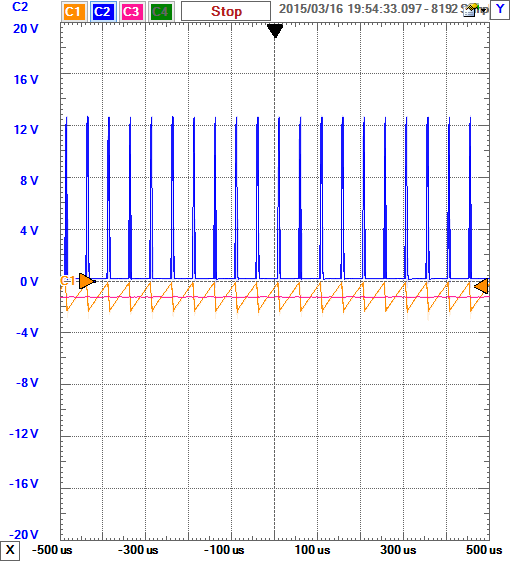
\includegraphics[scale=0.7]{img/circuit-test-1060mv.png}
	\caption{Test du circuit \unit{-1060}{\milli\volt}.}
	\label{fig:test-1060}
\end{figure}

\end{document}